\documentclass{project}
\usepackage[pdfauthor={L Jones},pdftitle={Software Engineering Group Project, Final Report},pdftex]{hyperref}
\usepackage{graphicx}
\usepackage[export]{adjustbox}
\usepackage{pdfpages}
\usepackage{longtable}
\graphicspath{ {images} }
\begin{document}
\title{Software Engineering Group Project}
\subtitle{Final Report}
\author{L. Jones, M. Goly, T. MIlls}     
\shorttitle{Final Report}
\version{1.2}
\status{Release}
\date{2016-02-15}
\configref{SE-12-FR}
\maketitle
\tableofcontents 
\newpage

\section{INTRODUCTION}
\subsection{Purpose of this document}
The purpose of this document is to outline that which we have achieved and gained as a group throughout the software development process, and to reflect on the process as a whole.

\subsection{Scope}
The document covers the process as a whole, including the state of the software produced, the standards set in our documentation as well as other non-technical aspects such as how we collectively worked as a team and how we could improve.

This document assumes the reader is familiar with the requirements specification\cite{se.qa.rs} and all of the quality assurance standards associated with the project.

\subsection{Objectives}
The objectives of this document are as follows:
\begin{itemize}
\item{To provide a concise summary on the state of the software including areas in which it could be improved.}
\item{Discuss the documentation produced and how it was necessary for it to be altered during the process.}
\item{Provide a general summary of the project on the whole from a historical point of view i.e. how?/when?/why? were things done.}
\item{Outline the roles and duties performed by every individual.}
\item{Provide a test log to illustrate where the software passed/failed our tests\cite{se.qa.ts}.}
\item{Produce a maintenance manual for the benefit of program maintainers.}
\end{itemize}
\clearpage

\section{END OF PROJECT REPORT}
\subsection{Management summary}
In terms of the software produced we believe we have completed what was required\cite{se.qa.rs} to a good standard. Our software adheres to all the necessary functions and requirements as proved during the acceptance testing, with the exception that TaskerMAN does not currently support filtering. This was not due to team members lacking the capability to implement the function, rather it was a misunderstanding when reading the requirements specification, it was only during acceptance testing that we realised we'd made the error. There are areas where the code could be cleaner e.g. the  `Syncer' class within TaskerCLI contains overly complex methods, which make the code more difficult to understand and potentially problematic for a future developer to maintain, though it is all functional. The front-end of TaskerCLI is also not the most eye-catching as we weren't able to design it completely as we wanted due to time constraints, however it's also completely functional.

From a documentation point of view we are also in good stead. On the whole we received positive remarks for both our Test Specification and Design Specification, receiving grades B- and A respectively. Based off the feedback received from both our project manager and project coordinator we made further improvements to the documentation where necessary. The Project Plan was also maintained and updated throughout the entirety of the project by the Group Leader.

The main obstacle of the project were the numerous bugs encountered with TaskerCLI during Integration and Testing Week. In particular, we had an issue where comments made related to the task elements of a task would not save when the task panel was closed, which was a major part of the functionality of the software. The issue stemmed from our naive implementation of merging the remote objects and the local objects. The way that our TeamMemberDB.updateTeamMember method was originally written meant that it would take the remote object, look at the list of tasks it has associated with it, then iterate through the list of tasks. We would then call the sql query UPDATE on tasks to update them, but this didn't work on the local copy of tasks. To fix this we had to change the update method to remove the team member, then re-insert into back into both of the databases, rather than just trying to update it. This solved the issue. There were other issues associated with TaskerCLI such as task reassignment not working, however these issues were much less time-consuming and less frustrating to solve than our main issue. There were also other problems that occurred which were out of our hands e.g. during Integration and Testing Week, we were unable to work for several hours due to a power failure on site, and one morning the remote database was not able to be written to, however such incidents were accounted for in the Risk Analysis of the Project Plan\cite{se.qa.pp}.

As a team we worked well together. From a documentation point of view everybody had an input. From a software development point of view there was a bit of an imbalance in terms of work load. Members of the TaskerCLI subteam naturally had more work due to the way in which we designed the system\cite{se.qa.ds} and the more technically proficient members of the group found themselves with the most work allocated to them. Though TaskerMAN was a relatively easy system to design in comparison, there was still the same issue of the most technically proficient member being allocated the most work which was unfair, and this was an error on my behalf (Luke Jones - Project Leader). However as a group the morale was generally good, there were no major personality clashes that hindered the project in any way and we worked effectively to achieve what was required of us.

\subsection{Historical account of the project}
The initial group meetings were concerned with familiarising each other as a team and the requirements specification. Shortly after this roles were allocated based on team member's strengths/weaknesses. 

The first major deliverable was the outline for the `Interaction and High-Level Design' of the system as part of the Design Specification document. Simultaneously it was required that the project Leader create a Project Plan with an accompanying Gantt Chart and Risk Analysis. After some initial confusion due to it being the first deliverable and team members being not used to the format of delivery, the `Interaction and High-Level Design' was completed, reviewed and submitted. As part of the document, we were required to create diagrams and a narrative for the application deployment i.e. applications interface and applications in the system, as well as use-cases for both TaskerMAN and TaskerCLI. It was also necessary for us to design the UI for TaskerMAN and TaskerCLI at this point, and the designs that we created in this period are very similar to the UI which exists on the finished product.

After this deliverable the head developer of TaskerMAN (Tino Garapasi) elected to begin work on prototypes of the website and presented them to the group. We were very impressed with what he'd made and the fact that he worked hard on the system in the beginning meant that our overall workload was significantly reduced later on in the project.

The next major delivery was the  `Test Specification'. The creation of tests and a test table was allocated largely to one individual (Tom Mills). We failed to have a review meeting for this document and consequently received a lower grade than our previous deliverable. Meanwhile members of the TaskerCLI subteam began work on a TaskerCLI prototype. The major implementation in this prototype was the `Syncer' class related to the synchronisation aspect, which was a difficult class to code, along with all the other necessary functionalities required for the prototype demonstration to our project manager.

The next deliverable required was the complete  `Design Specification', which was a continuation of the  `Interaction and High-Level Design' deliverable in more detail, including sections such as  `Significant Classes" and  `Detailed Design', both of which required several sub-sections and numerous diagrams with pieces of narrative. This document was completed, reviewed and submitted and received positive feedback.

The final delivery of the first term was the actual prototype demonstration to our project manager of a working system. TaskerMAN was already nearly fully-functional at this point, and the TaskerCLI subteam worked hard during the final week to prepare it for demonstration. On the final day we solved several critical bug issues related to the prototype and had several practice demonstration before finally showing our project manager our progress. He was very pleased with the system and praised us on our progress. Up to this point the process strictly followed a plan as there were no major setbacks.

The next time we convened for group project duty was Integration and Testing Week, which was a long time after the prototype demonstration due to Christmas and an exam period. We began the week by creating a list of all known functionality issues on TaskerMAN and TaskerCLI and creating GitHub issues for each individual issue. From a TaskerMAN point of view the major tasks included implementing the optional feature of authentication and cleaning up the website on the front-end. From a TaskerCLI point of view the goal was on fixing any pre-existing bugs and to implement any functional requirements which had not yet been implemented.

The TaskerMAN development ran relatively smoothly and according to plan. We were able to implement everything that we wanted, the front-end was cleaned up and we were able to test the website on a non-developer (Tom Mills) to test it's user-friendliness, and all tests were passed. All tests related to TaskerMAN as outlined in the  `Test Specification'\cite{se.qa.ts} in terms of functional requirements also passed. On the final day we completed the installer and it's associated README.txt and we were very satisfied with the final system.

TaskerCLI development was not as smooth. The target was to spend 3 days fixing critical bugs and implementing a cleaner UI, before moving onto testing and the installer. What actually happened was that the vast majority of the week was spent fixing critical back-end e.g. as comments made to task elements not saving. Because of this there wasn't any opportunity to clean up the UI, although it's still relatively user friendly as it passed the UI tests outlined in the  `Test Specification'. The final system also passed all of the functional requirements associated with it in the 'Test Specification'. On the final day there were difficulties implementing the installer due to the way our system was designed\cite{se.qa.ds} however it was ultimately completed and it's associated README.txt written. Although such problems as the ones encountered when developing were accounted for in the Risk Analysis TaskerCLI's development was often frustrating due to the fact we didn't achieve 100\% of what we wanted.

Acceptance testing began a few days later. Our software passed all of the tests, however as explained earlier failed the filtering requirements of TaskerMAN due to team members misunderstanding the requirements specification.

It was now time for team members to draft their personal reflective report and work on the final deliverable  `Final Report', including the  `End-of-Project Report',  `Test Report' and `Maintenance Manual'. These were completed and complied shortly before the deadline. At this point we also confirmed that everything was in good order on our repository as outlined in the `Operating Procedures and Configuration Management Standards' quality assurance document, and confirmed `nwh-aber' was a collaborator on the repository.

Throughout the entirety of the project team members maintained a weekly blog outlining their progress and contribution.
\subsection{Final state of the project}
All of the necessary functional requirements of Tasker have been implemented with the exception of filtering in TaskerMAN. TaskerMAN currently supports the sorting of tasks when viewing tasks, either by expected completion date (default), member assigned to or task status, but not full filtering as required \cite{se.qa.rs}. Also in the README.txt file of the TaskerMAN there is no mention of the need to change permissions (if necessary). Finally the TaskerCLI installation script should also be moved from the src folder to TaskerCLI\_Installation. All of the documentation is in good standing, has been updated based on the feedback received during the process and is correctly documented with regards to referencing and document change history. 

\subsection{Location of the group repository}
The URL of our repository is https://github.com/MichalGoly/Tasker. Within our \textit{src} folder TaskerCLI is a submodule with the URL https://github.com/MichalGoly/TaskerCLI. The final branch for delivery is the default \textit{master} branch. The user `nwh-aber' is both a collaborator on the main Tasker repository and the TaskerCLI submodule.

\subsection{Performance of each team member}
\subsubsection{Adam Neaves}
Adam Neaves was a member of the TaskerCLI subteam, specifically the front-end development. Adam was tasked with designing the front-end of the client which he did as seen in the Design Specification\cite{se.qa.ds}. The current working TaskerCLI is pretty similar to the design as seen in the Design Specification, though it's not quite as clean or eye-catching and lacks the colour. This was due to unforeseen errors on the back-end of TaskerCLI meaning that we had to reallocate resources to solving critical issues, though the front-end design is still very user-friendly. During Integration and Testing Week he diverted his focus to fixing errors that existed on the TaskerCLI prototype, as well as single-handedly writing the Javadoc comments for almost all of the TaskerCLI code. From a documentation point of view he played a vital role on the detailed design section of TaskerCLI in the Design Specification, in particular creating a number of extremely informative sequence diagrams with explanation. He was also responsible for the production of the TaskerCLI use-case diagram and narrative.

Adam had a good working relationship with all members of the group and completed all the tasks allocated to him. During group meetings he would always contribute with valuable input and was happy to explain anything to the other group members if they were struggling to understand as he was always aware of what needed to be achieved. In his own words Adam feels he could've played a more instrumental role during Integration and Testing Week, however due to back-end issues with TaskerCLI this wasn't possible and was certainly through no fault of his own.
\subsubsection{Josh Mir}
Josh Mir was the Deputy Project Leader. He was also a key developer on the TaskerCLI application as he had prior experience working with Java development. From a deputy project leader point of view he wasn't required to do anything as the project leader didn't assign him any tasks associated with the management of the project, and he wasn't required at any point to lead the project in the project leader's absence. Josh worked alongside Michal on the back-end development of TaskerCLI, implementing the most challenging aspects of the design\cite{se.qa.ds} such as synchronisation between the local and remote databases. He was key in solving a number of critical bugs we encountered during Integration and Testing Week for TaskerCLI, as well as helping the TaskerMAN subteam with any issues they were having. He also assisted on the TaskerMAN side of the project during design, suggesting that we use a Bootstrap template for a slick and simple design, which we did. He was the most knowledgable with operating Git, and was responsible for setting up TaskerCLI as a submodule within the \textit{src} folder of the Tasker repository. He also assisted with the TaskerCLI installer and it's associated README.txt.

Josh had a good working relationship with all members of the group, was highly approachable with any issues team members were having and had a high level of technical proficiency related to all aspects of the project, not just Java and TaskerCLI.
\subsubsection{Luke Jones}
Luke Jones was the Project Leader. He moderated group meetings, booked rooms for group meetings and was the main means of communication between the group and project manager. From a technical point of view he was a member of the TaskerMAN subteam as he had prior experience with HTML/PHP. During Integration and Testing Week he worked mainly on the front-end of TaskerMAN, correcting issues that made the site less eye-catching, as well as spotting a number of bugs associated with the front-end of the site e.g. the date picker wasn't originally responsive in Firefox or Safari browsers. He also had a minor input on the back-end of the website, assisting the main developer (Tino) with any errors which occurred. He also assisted with the installer for TaskerMAN and helped write the README.txt for installation. He played a larger role from a documentation point of view, working largely on the TaskerMAN elements of the Design Specification, as well as being the person responsible for compiling everyone's sections together for delivery. He also maintained a Project Plan throughout the entirety of the process.

Luke was largely organised in what he did, and maintained group harmony to the best of his ability. He never missed a meeting and always had an agenda prepared beforehand. He was very approachable and had a good relationship with the other members of the group. An area in which he could improve is that he could've more equally allocated work during Integration and Testing Week as it was quite imbalanced which led to frustrating and unfair situations.
\subsubsection{Michal Goly}
Michal Goly was the head developer of the TaskerCLI application as his strengths lied in Java development. He worked incredibly hard on the back-end of the client, both during and prior to Integration and Testing Week, as due to the way our system was designed\cite{se.qa.ds} it was a complex and error-prone Java application. During group meetings Michal would play a very active role in discussion and being the overall most technically proficient member of the team, always contributed valuable input. During Integration and Testing Week a large part of his time was devoted to solving the numerous issues that existed on the TaskerCLI prototype, as most of the features had already been implemented, as well as working on the installer for TaskerCLI and it's associated README.txt. From a documentation point of view he also played a valuable role, in particular in the Design Specification on the deployment description and TaskerCLI detailed design sections, as well as contributing to the maintenance manual in the Final Report.

Michal worked tirelessly for the group and was extremely determined. He was always aware of his duties and would often help others in their own tasks. He arguably had the biggest contribution to the project alongside Josh and Tino. Michal had a good relationship with all members of the group.
\subsubsection{Will Jones}
Will Jones was a member of the TaskerMAN subteam. Will's roles and duties we're identical to mine (Project Leader) without the management work. Early in the process he assisted Tino with the narrative for TaskerMAN UI in the Design Specification\cite{se.qa.ds}, and also put a lot of work into the detailed design of TaskerMAN e.g. wrote the entire signifcant classes section for TaskerMAN. During Integration and Testing Week Will worked on the already functional prototype and made mostly front-end changes, e.g. CSS alterations to make the site more user-friendly and savvy safety features such as changing password fields to print out asterisks instead of plain text. He worked alongside Tino on the authentication aspect helping to create the login/logout functions. He was also tasked with formatting and commenting on our TaskerMAN code.

Will had a good working relationship with all members of the team and was very approachable when asked to complete a task. He seldom missed a meeting and if unsure of something technical then he would work hard to make sure he understood it eventually.
\subsubsection{Tino Garapasi}
Tino Garapasi was the head developer of TaskerMAN. He was also originally the deputy quality assurance officer however during the process that resposibility was handed to Tom Mills as Tino no longer desired the role. Tino played a massive role in the early stage of TaskerMAN development, creating the majority of the prototype single-handedly. During Integration and Testing Week Tino's work consisted of fixing any back-end issues that existed with the site e.g. protecting the site from SQL injection. He was also the primary person involved with creating the TaskerMAN installer and the associated README.txt. He played a very active role in the documentation,  in the Design Specification\cite{se.qa.ds} he created TaskerMAN use-case diagrams and TaskerMAN object diagrams, as well as the TaskerMAN component description.

Tino had a good working relationship with all members of the team and was very easy to work alongside. The hard work he did early on in the process significantly aided us in Integration and Testing Week from a TaskerMAN point of view. He always completed what was asked of him and would often work relentlessly for the benefit of the group, and wouldn't hesitate to help a member of the team who required assistance.
\subsubsection{Tom Mills}
Tom Mills was the Deputy Quality Assurance. He wasn't originally however after Tino no longer desired the role he volunteered himself. From a quality assurance point of view the only responsibility he had was to take and upload the minutes when the quality assurance officer was absent. Tom's main role was in the team was tester. He contributed massively in this aspect, creating most of the Test Specification by himself maintaining it based on the feedback received. During Integration and Testing Week he was responsible for the testing of the TaskerCLI application, creating unit tests throughout the week, as well as helping the TaskerCLI subteam with issues in any way he could due to Java development being one of his strengths. He was also responsible for the Project Test Report which appears in this report. He worked on the Design Specification\cite{se.qa.ds} writing a narrative with regards to spike programming.

Tom had a good working relationship with all members of the group. He participated in every meeting, offered input where he could and completed everything that was requested of him. It probably wasn't a good idea for such a large aspect of the process (testing) to be allocated to one individual however this was an error on my part (Project Leader).
\subsubsection{Tom Oram}
Tom Oram was the Quality Assurance Officer. Tom was responsible for taking the minutes of every meeting, and uploading them to GitHub, which after some initial trouble with Git, he did consistently and on time. During Integration and Testing Week he was a part of the testing team, in particular as he was a non-developer of the TaskerCLI application he was able to test the user-friendliness of the application to the average user. He checked the code created by the TaskerCLI subteam to ensure it complied with the Java coding standards as outlined\cite{se.qa.jcs}. He also assisted the TaskerMAN subteam with certain CSS issues they were having such as divs not correctly centering. He had the final say on documentation, and approved them before they were ready for release. He assisted in the moderation of review meetings alongside the project leader.

Tom was a friendly member of the group and had a good relationship with all the other team members. He completed every task which was assigned to him, and being an all-rounder assisted others in any way he could. He found himself with less work than expected in terms of documentation as I (Project Leader) would naturally check everything was in order while compiling everyone's sections together, therefore the amount of input he could possibly have here was limited.

\subsection{Critical evaluation of the team and the project}
On the whole we performed well as a team. We became comfortable with one another early on in the process, we were aware of each others strengths/weaknesses after an initial meeting and there were no major personality clashes. Roles were allocated very early on in the process and these did not change, with the exception of the deputy quality assurance changing from Tino to Tom Mills as he longer wanted the role. This contributed to a productive work environment. Early on in the process work was divided relatively equally amongst the group as a large part of the work was documentation and initial design. During the latter stages of the process the workload became slightly imbalanced as the more technically proficient members of the team were allocated the most work, particularly during Integration and Testing Week. This created a sense of frustration amongst some team members, lowering the overall morale and team chemistry. To combat this in future the work load should be shared more equally to create a less stressful environment, which in turn might lead to better results from a technical point of view. We were however quite fortunate with our group allocation, in that we had specialists in all the necessary areas of the project, meaning team members usually knew exactly what they were and weren't responsible for. At no point during the process was it necessary for a team member to be punished, either by the project leader or the project manager.

There are a few suggestions we have as to how the project process could be improved. Some team members had great difficulty in using Git as they had no prior experience, leading to situations where some team members would have to upload to the repository on behalf of other members. Though there was an introductory session to Git at the beginning of the year, this clearly wasn't enough, so maybe Git tutorials could be provided during the first year in order to give students a head start. Also the hand-in dates for many of the major documentation deliverables coincided with the hand-in dates for major assignments of other modules. Whilst understandably this may be unavoidable, it meant that we had to compromise on the amount of resources we could dedicate to the group project. 

We've learned many valuable lessons about the software development life cycle during this process. The major one being that you must be prepared for setbacks. During Integration and Testing Week, we had numerous issues with TaskerCLI bugs, some critical, which took longer than desired to fix, meaning that less resources could be allocated to other aspects of the process such as system testing. While this was accounted for in the Risk Analysis of the Project Plan\cite{se.qa.pp} it certainly created a sense of frustration. Another is the importance of review meetings to the quality of documentation. For the Test Specificaition for which we initially didn't have a formal review our grade was considerably lower (B-) than that of our Design Specification (A), for which we did have a review meeting.
\clearpage

\section{PROJECT TEST REPORT}
Here is the final project test report of our project made during Integration and Testing Week. All of our tests passed therefore the table is very clear. The tests outlined in this report are derived from our Test Specification\cite{se.qa.ts}. \\

\textbf{Group 12} \\
\textbf{Test log: 002} \\
\textbf{Date: 28/01/2016} \\

\begin{longtable}{| p{1.8cm} | p{2.5cm} | p{2.5cm} | p{8.5cm} |}
\hline
Task ID & Tester & Pass/Fail &  Fail Comments \\
\hline
MAN-001 & T. Mills & Pass & N/A \\
\hline
MAN-002 & T. Mills & Pass & N/A \\
\hline
MAN-003 & T. Mills & Pass & N/A \\
\hline
MAN-004 & T. Mills & Pass & N/A \\
\hline
MAN-005 & T. Mills & Pass & N/A \\
\hline
MAN-006 & T. Mills & Pass & N/A \\
\hline
MAN-007 & T. Mills & Pass & N/A \\
\hline
MAN-008 & T. Mills & Pass & N/A \\
\hline
MAN-009 & T. Mills & Pass & N/A \\
\hline
MAN-010 & T. Mills & Pass & N/A \\
\hline
MAN-011 & T. Mills & Pass & N/A \\
\hline
MAN-012 & T. Mills & Pass & N/A \\
\hline
MAN-013 & T. Mills & Pass & N/A \\
\hline
MAN-014 & T. Mills & Pass & N/A \\
\hline
MAN-015 & T. Mills & Pass & N/A \\
\hline
MAN-016 & T. Mills & Pass & N/A \\
\hline
MAN-017 & T. Mills & Pass & N/A \\
\hline
CLI-001 & T. Mills & Pass & N/A \\
\hline
CLI-002 & T. Mills & Pass & N/A \\
\hline
CLI-003 & T. Mills & Pass & N/A \\
\hline
CLI-004 & T. Mills & Pass & N/A \\
\hline
CLI-005 & T. Mills & Pass & N/A \\
\hline
CLI-006 & T. Mills & Pass & N/A \\
\hline
CLI-007 & T. Mills & Pass & N/A \\
\hline
CLI-008 & T. Mills & Pass & N/A \\
\hline
CLI-009 & T. Mills & Pass & N/A \\
\hline
CLI-010 & T. Mills & Pass & N/A \\
\hline
CLI-011 & T. Mills & Pass & N/A \\
\hline
CLI-012 & T. Mills & Pass & N/A \\
\hline
CLI-013 & T. Mills & Pass & N/A \\
\hline
CLI-014 & T. Mills & Pass & N/A \\
\hline
UI-001 & T. Oram & Pass & N/A \\
\hline
UI-002 & T. Oram & Pass & N/A \\
\hline
UI-003 & T. Oram & Pass & N/A \\
\hline
UI-004 & T. Oram & Pass & N/A \\
\hline
UI-005 & T. Oram & Pass & N/A \\
\hline
UI-006 & T. Oram & Pass & N/A \\
\hline
UI-007 & T. Oram & Pass & N/A \\
\hline
UI-008 & T. Oram & Pass & N/A \\
\hline
UI-009 & T. Oram & Pass & N/A \\
\hline
UI-010 & T. Oram & Pass & N/A \\
\hline
UI-011 & T. Oram & Pass & N/A \\
\hline
UI-012 & T. Oram & Pass & N/A \\
\hline
UI-013 & T. Oram & Pass & N/A \\
\hline
UI-014 & T. Oram & Pass & N/A \\
\hline
UI-015 & T. Oram & Pass & N/A \\
\hline
PER-001 & T. Mills & Pass & N/A \\
\hline
PER-002 & T. Mills & Pass & N/A \\
\hline
PER-003 & T. Mills & Pass & N/A \\
\hline
PER-004 & T. Mills & Pass & N/A \\
\hline
PER-005 & T. Mills & Pass & N/A \\
\hline
PER-006 & T. Mills & Pass & N/A \\
\hline
PER-007 & T. Mills & Pass & N/A \\
\hline
PER-008 & T. Mills & Pass & N/A \\
\hline
PER-009 & T. Mills & Pass & N/A \\
\hline
\end{longtable}

For reference, here are relevant parts that failed on a previous test log where there was an issue connecting TaskerCLI to the remote database. \\

\textbf{Group 12} \\
\textbf{Test log: 001} \\
\textbf{Date: 27/01/2016} \\

\begin{longtable}{| p{1.8cm} | p{2.5cm} | p{2.5cm} | p{8.5cm} |}
\hline
Task ID & Tester & Pass/Fail &  Fail Comments \\
\hline
CLI-001 & T. Mills & Fail & Error message popped up. User Not in the Database, connected to local database.  \\
\hline
CLI-002 & T. Mills & Fail & Error message popped up, incorrect details.  \\
\hline
CLI-003 & T. Mills & Pass & N/A \\
\hline
CLI-004 & T. Mills & Fail & Login details not stored in local database, did not login and sync to the local database.  \\
\hline
CLI-005 & T. Mills & Fail & Task list not displayed, could not log in. \\
\hline
CLI-006 & T. Mills & Fail & See error message for task CLI-005  \\
\hline
CLI-007 & T. Mills & Fail & Could not delete task, no tasks displayed.  \\
\hline
CLI-008 & T. Mills & Fail & Could not complete a task, no tasks displayed.  \\
\hline
CLI-009 & T. Mills & Fail & Could not edit a task, no tasks displayed.  \\
\hline
CLI-010 & T. Mills & Fail & See error message for task CLI-009  \\
\hline
CLI-011 & T. Mills & Fail & Could not synchronise, Js@smith.com could not log in.  \\
\hline
CLI-012 & T. Mills & Fail & See error message for task CLI-011  \\
\hline
CLI-013 & T. Mills & Fail & Could not view tasks, no tasks displayed.  \\
\hline
CLI-014 & T. Mills & Fail & Could not log in, could not sync after 5 minutes. \\
\hline
\end{longtable}
\clearpage

\section{PROJECT MAINTENANCE MANUAL}
\subsection{Program description}
TaskerMAN is the website application for Tasker. Users are able to maintain a session on the site as PHP authentication is a feature. Users are able to create both task data and team member data, which is stored in TaskerSRV. Users are also able to edit both task and team member data, as changes are written to TaskerSRV.

TaskerCLI is the Java application for Tasker. Users login with their email and password as set on TaskerMAN. They're then able to view the tasks which have been allocated to them, which are listed in order of their `taskid' which is a unique attribute given to every task in TaskerSRV upon task creation. Clicking on a task displays elements associated with the task which are displayed in the order they were produced on TaskerMAN. Comments can be made on task elements, which upon synchronisation will write the comment to TaskerSRV.
\subsection{Program structure}
Information is contained within the Design Specification\cite{se.qa.ds}.

\subsection{Algorithms}
Information is contained within the Design Specification\cite{se.qa.ds}.

\subsection{The main data areas}
Information is contained within the Design Specification\cite{se.qa.ds}.

\subsection{Files}
Information is contained within the Design Specification\cite{se.qa.ds} A local SQLite database will be required for storage.

\subsection{Suggestions for improvements}
\begin{itemize}
  \item Front end of the TaskerCLI has been developed using Swing. Initially we had
    designed the list of the tasks for the logged in user, as a list of generated
    JPanel components, rather than the JTable that we have used eventually. This would
    have allowed us to create a richer and more interesting user interface. 
  \item When user selects one of the tasks in the TaskerCLI, the TaskFrame dialog 
    is opened to allow the user to comment on his progress on the clicked task. However
    in order to save newly created comment, he has to manually press enter before closing
    the window. This behaviour has a negative impact on the user-friendliness, and could
    be improved by allowing the user to edit the comment box and press the Complete/Close
    button on the bottom of the screen, without having to press  `ENTER' beforehand.
  \item Some refactoring of TaskerCLI code may be needed in order to make the system more
    understandable. Especially the  `Syncer' class which has overly complex methods which
    could be further split to improve readability. For example the logIn method, not
    only deals with the logical part of this operation, but also generates the login
    box for user's credentials. Ideally each method should only be responsible for 
    a single task, so login box presenting method could be introduced.
  \item The list of all the tasks in the system in TaskerMAN can be currently sorted
    by the completion date, the status of the task and the member that has been assigned
    to the task. Tasks filtering could be implemented to improve the usability of the
    system. User could then filter tasks by their status or the member assigned, instead
    of sorting which still requires the manager to scroll through multiple results as stated in the requirements specification\cite{se.qa.rs}. 
  \item A friendly message could me implemented in TaskerMAN to inform the user if there
    is a problem with accessing the remote database. Currently, TaskerMAN user interface
    is loaded without the data which makes the system appear less professional. 
  \item Currently it is impossible to enter tasks into the system with names containing
    special characters like apostrophes. This prevents SQL injections, but has an impact
    on the usability of the system. A more sophisticated approach to preventing SQL injections
    and XSS attacks could be implemented.
  \item It's currently not possible to add a task in TaskerMAN with the same name as another pre-existing task due to the task title being a unique attribute in TaskerSRV.
  \item Finally README with the instructions to install TaskerMAN could be updated with
    the information about the necessary change of permissions in order for the system
    to work. TaskerCLI installation script should also be moved from the src folder 
    to the TaskerCLI\_Installation. 
\end{itemize}

\subsection{Things to watch for when making changes}
In an application of this size, it is inevitable that a change to one part of the system
can brake something else. It is therefore essential to back up the original
version of the system before attempting to fix or improve anything. Version control 
system like git seems to be an obvious and recommended approach.

Due to the way Data Object Access pattern has been used, any changes to the database
structure (TaskerSRV) will require significant changes to both the 
\texttt{uk.ac.aber.cs221.group12.taskercli.business} and 
\texttt{uk.ac.aber.cs221.group12.taskercli.data} TaskerCLI packages. Within the business
package, JavaBean entities abstract the tables within the database. Therefore if you
make a change to the underlying database, you have to make changes in appropriate 
entities as well. Same problem applies to the data package. Because within the front end
of the program, developer can access a given TeamMember object by its email, quite
possibly the whole chain of method calls that rely on each other may have to be changed,
along with the SQL queries on the top of each file. 

Developers have to be especially careful when making any changes to the synchronisation
part of the TaskerCLI. Before making any changes it is advisable to refer to the
Design Specification\cite{se.qa.rs} to understand how this behaviour
is achieved. The main concept is fairly straightforward: you retrieve the remote TeamMember
object, retrieve the locally stored TeamMember object, merge them together and finally 
login and use its data to populate the view. Things however become quickly more complex, when
you consider all the possible scenarios like lack of the Internet connection and the precedence
of different information about the team member (e.g. task list on the remote database takes
precedence over the local version, but comments to any existing tasks have to be taken
from the local one).

From a TaskerMAN perspective there exist many variables that span across several .php files e.g. the variable \$Username is present on every page (except for login.php) as it's echoed on the top menu bar of every page. If you were to alter this variable where it's initialised in login.php, then you would have to alter it across all the pages. Developers must also be wary of editing the connector.php file. Since this file is responsible for accessing the TaskerSRV changing the database login credentials will mean that none of the data present in TaskerSRV will be displayed. This may be desirable if you have a different database you'd rather connect to, however the new database would have to have exactly the same tables and table names as the ones present in TaskerSRV.
\subsection{Physical limitations of the program}
Tasker system requirements:
\begin{itemize}
  \item Apache web server capable of running PHP to deploy TaskerMAN.
  \item Pre-installed MySQL instance running either alongside the Apache web server, or
    separately to install TaskerSRV.
  \item Personal computer running any operating system capable of running Java Runtime
    Environment 7 or above to install TaskerCLI.
\end{itemize}
\subsection{Rebuilding and Testing}
The whole system can be run and tested locally, provided developer has access to 
locally running MySQL and Apache. For instance if Ubuntu OS is used for development,
both these requirements can be installed after a quick search through the Internet.
Having installed Apache and MySQL, developer needs to acquire the whole source code
of the program and follow the installation guide provided in order to deploy each
of the components.
\begin{itemize}
  \item TaskerMAN part of the system can easily be edited by changing the contents of
    PHP source files.
  \item TaskerSRV can be edited by editing the SQL script which builds the initial structure
    of the database. Whenever you need to revert the database state back to its original 
    state, you should follow the TaskerSRV installation guide and run the SQL script
    against the installation of your MySQL database.
  \item TaskerCLI can easily be edited using any IDE capable of importing Maven projects.
    You can import the whole project by selecting the \texttt{pom.xml} file, which 
    describes the whole build and contains details about TaskerCLI dependencies. After the
    initial import, it is advisable to select the "build and clean" option within the IDE.
    This will download all the required dependencies and run all the JUnit tests inside
    the test package. If you have a problem with accessing either your local or remote
    database, please make sure the properties files with MySQL and SQLite connection
    details are pointing at your database and SQLite db file. 
\end{itemize}
\clearpage

\addcontentsline{toc}{section}{REFERENCES}
\begin{thebibliography}{12}
\bibitem{se.qa.rs} \emph{Software Engineering Group Projects}
Requirements Specifications.
N. W. Hardy, SE.QA.RS. 1.1 Release.
\bibitem{se.qa.ts} \emph{Software Engineering Group Projects}
Test Specification.
L. Jones, T. Oram, W. Jones, T. Mills, 1.1 Release.
\bibitem{se.qa.ds} \emph{Software Engineering Group Projects}
Design Specification.
L. Jones, T. Oram, T. Garapasi, M. Goly, W. Jones, A. Neaves, J. Mir, T. Mills, 1.9 Release.
\bibitem{se.qa.pp} \emph{Software Engineering Group Projects}
Project Plan.
L. Jones, 1.2 Release.
\bibitem{se.qa.jcs} \emph{Software Engineering Group Projects}
Java Coding Standards.
C. J. Price, A. McManus, SE.QA.09. 17 Release.
\end{thebibliography}

\addcontentsline{toc}{section}{DOCUMENT HISTORY}
\section*{DOCUMENT HISTORY}
\begin{tabular}{|l | l | l | p{8cm} |l | }
\hline
Version & CCF No. & Date & Changes made to Document & Changed by \\
\hline
1.0 & N/A & 2016-02-13 & Initial creation & M.Goly [mwg2] \\
\hline
1.1 & N/A & 2016-02-14 & Included End-of-project report and added Project Plan, Design Specification and Test Specification as appendices & L.Jones [luj9] \\
\hline
1.2 & N/A & 2016-02-14 & Included Project Test Report & L.Jones [luj9] \\
\hline
\end{tabular}
\label{thelastpage}

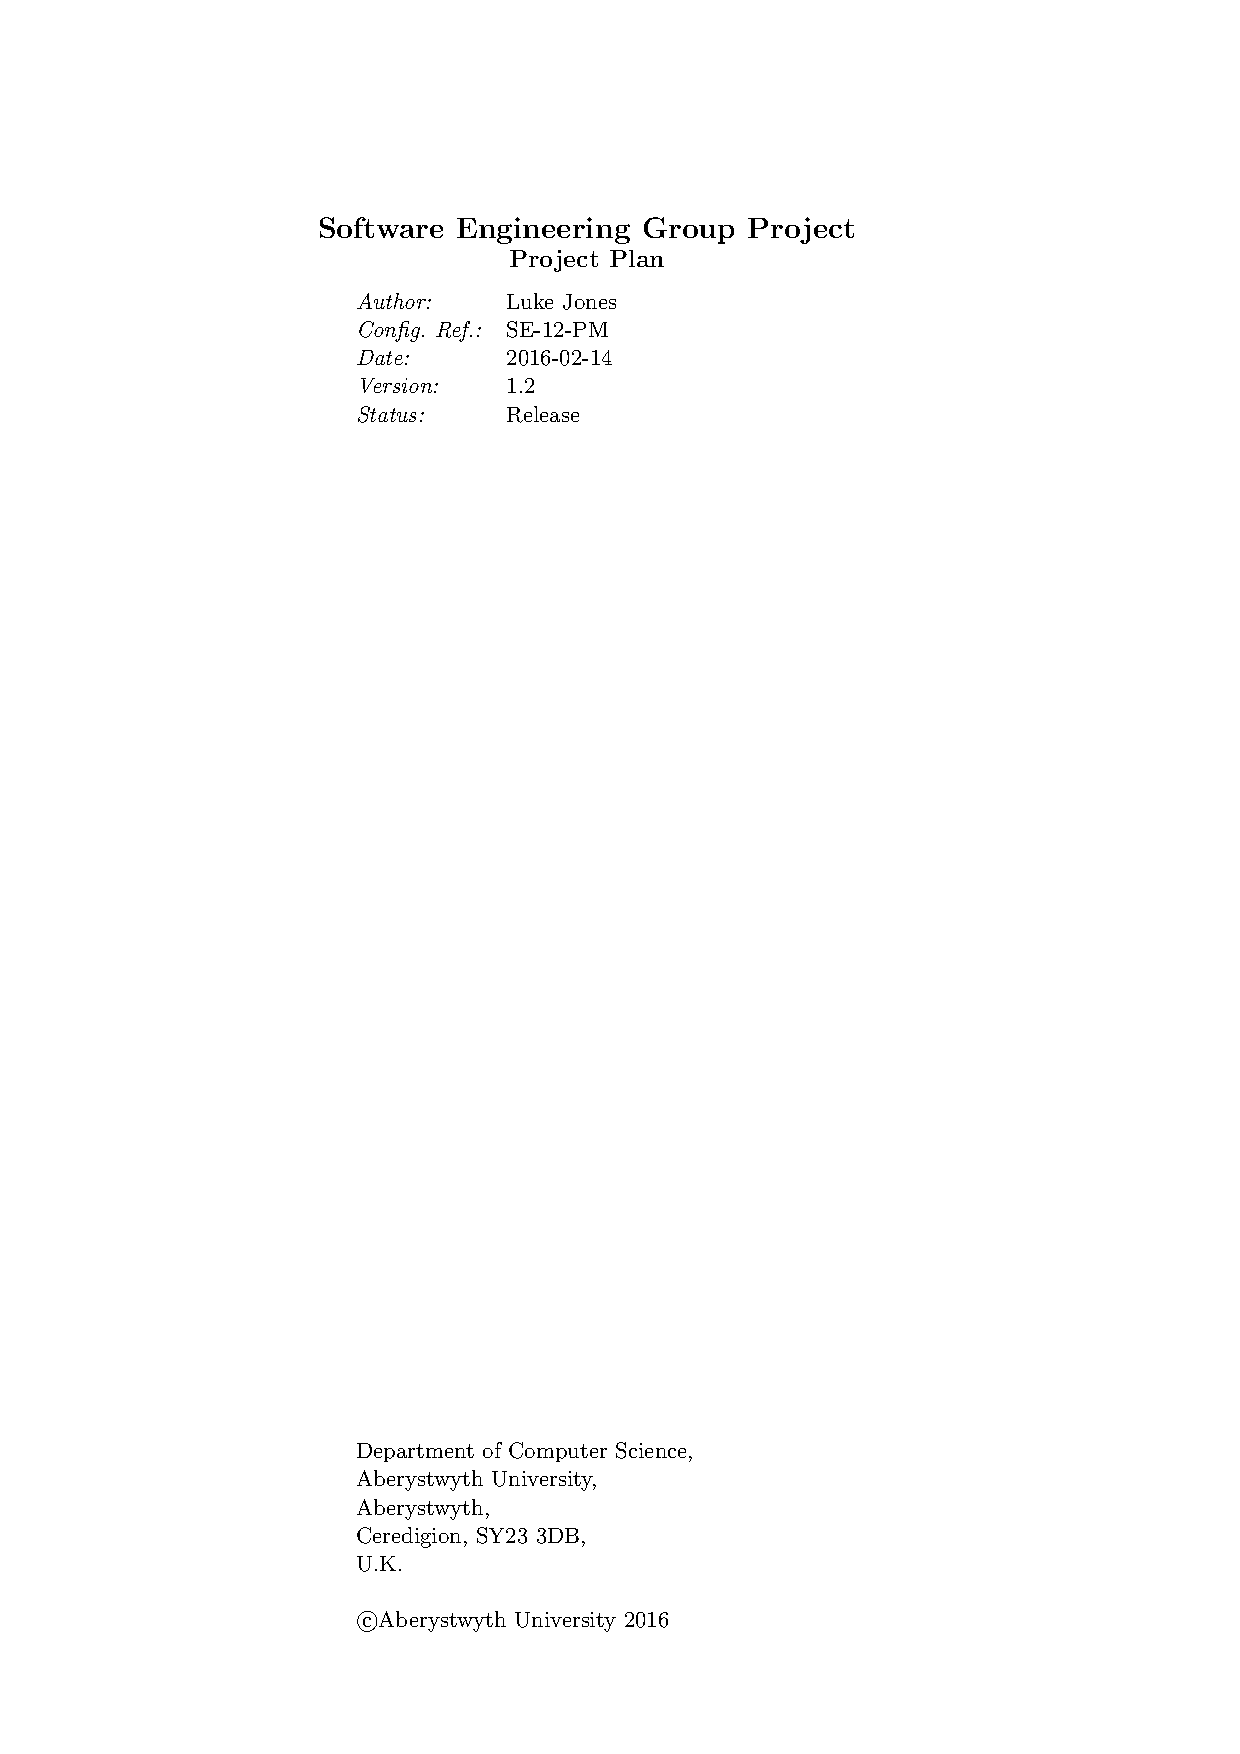
\includepdf[pages=-]{Project-Plan.pdf}
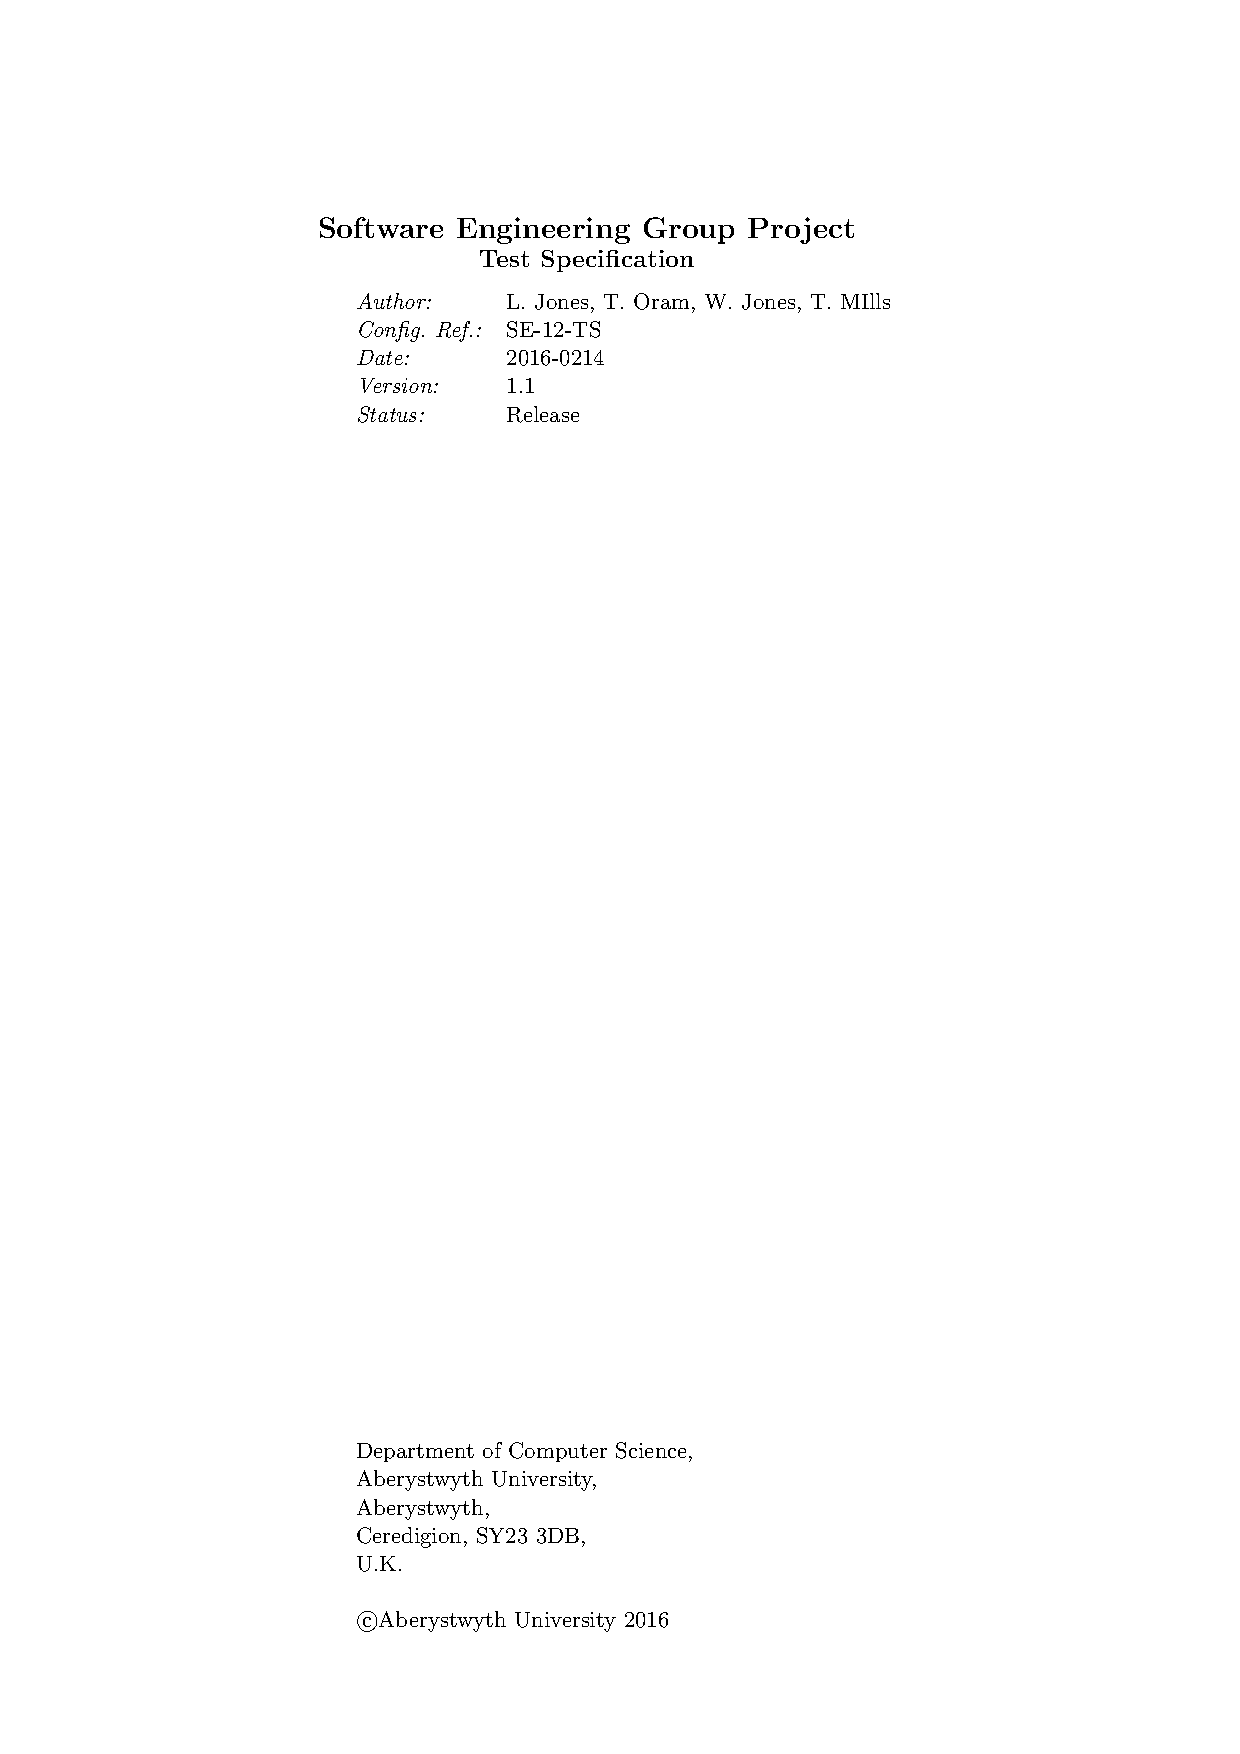
\includepdf[pages=-]{Test-Specification.pdf}
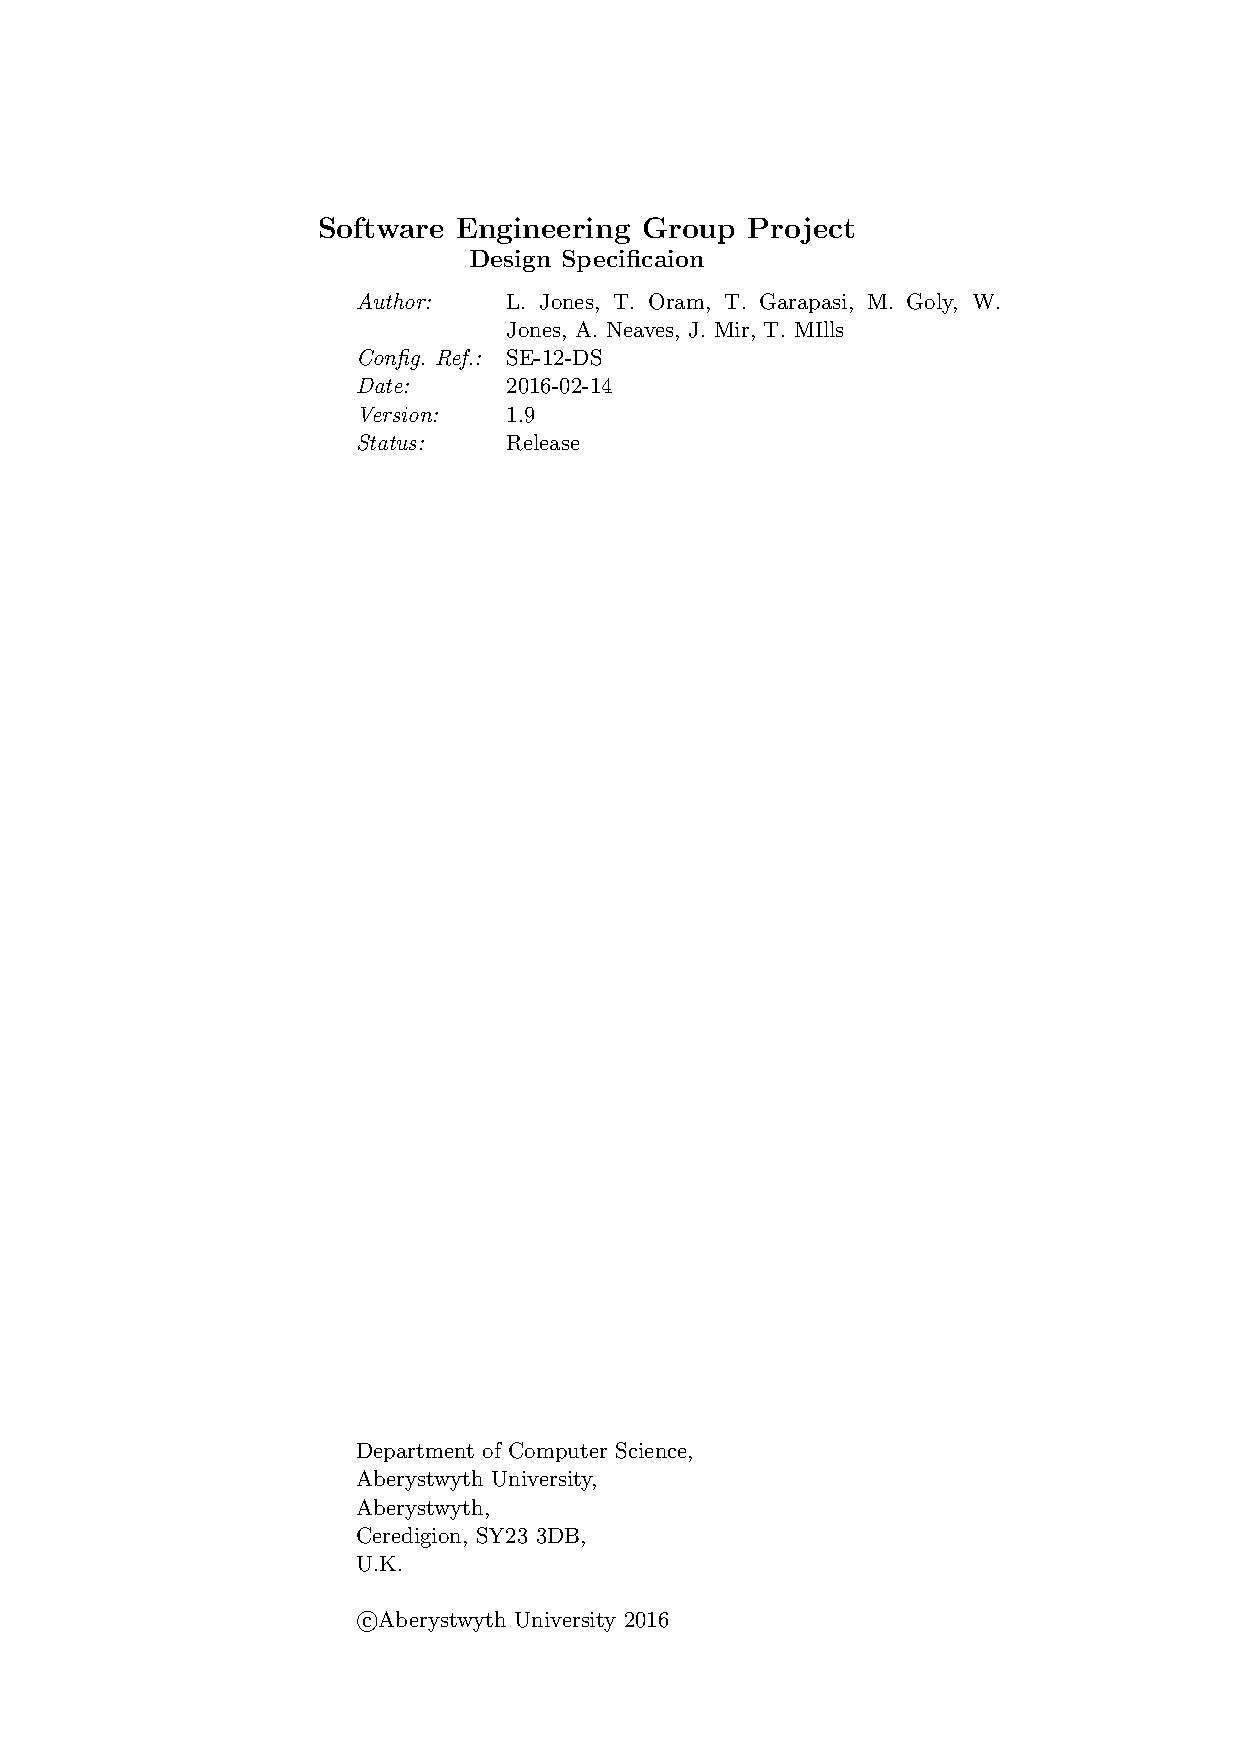
\includepdf[pages=-]{Design-Specification.pdf}

\end{document}
\end{verbatim}
\label{fig:footer}
\end{figure}
\label{thelastpage}
\end{document}